\section*{Цель}

Оценка и исследование дисциплин обслуживания потоков процессов при планировании их исполнения на основе приоритетных дисциплин с относительными и абсолютными приоритетами.

\section*{Исходные данные}

Данные из таблиц \ref{table:1}-\ref{table:4} являются исходными данными для выполнения лабораторной работы.

\begin{table}[H]
	\renewcommand{\tablename}{Таблица}
	\caption{Интенсивности поступления потоков обслуживаемых процессов}
	\begin{tabularx}{1\textwidth}{
			| >{\centering\arraybackslash}X
			| >{\centering\arraybackslash}X
			| >{\centering\arraybackslash}X
			| >{\centering\arraybackslash}X
			| >{\centering\arraybackslash}X
			| >{\centering\arraybackslash}X
			| >{\centering\arraybackslash}X
			| >{\centering\arraybackslash}X
			| >{\centering\arraybackslash}X
			| >{\centering\arraybackslash}X
			| >{\centering\arraybackslash}X |
		}
		\hline
		\multirow{2}{*}{\rotatebox[origin=c]{90}{№ варианта}} & \multirow{2}{*}{\rotatebox[origin=c]{90}{№ потока}} & \rotatebox[origin=c]{90}{Интенсивность потока} & \multirow{2}{*}{\rotatebox[origin=c]{90}{№ потока}} & \rotatebox[origin=c]{90}{Интенсивность потока} & \multirow{2}{*}{\rotatebox[origin=c]{90}{№ потока}} & \rotatebox[origin=c]{90}{Интенсивность потока} & \multirow{2}{*}{\rotatebox[origin=c]{90}{№ потока}} & \rotatebox[origin=c]{90}{Интенсивность потока} & \multirow{2}{*}{\rotatebox[origin=c]{90}{№ потока}} &
		\rotatebox[origin=c]{90}{Интенсивность потока} \\
		\cline{3-3}\cline{5-5}\cline{7-7}\cline{9-9}\cline{11-11}
		& & [1/c] & & [1/c] & & [1/c] & & [1/c] & & [1/c] \\
		\hline
		7 & 7 & 0,20 & 14 & 0,40 & 10 & 0,05 & 19 & 0,05 & 1 & 0,20\\
		\hline
	\end{tabularx}\label{tab:table2}
\end{table}

\begin{table}[H]
	\renewcommand{\tablename}{Таблица}
	\caption{Параметры обслуживаемых процессов.}
	\begin{tabularx}{1\textwidth}{
			| >{\centering\arraybackslash}p{1cm} | >{\centering\arraybackslash}p{5.7cm} | >{\centering\arraybackslash}p{0.5cm} | >{\centering\arraybackslash}p{0.5cm} | >{\centering\arraybackslash}p{0.5cm} | >{\centering\arraybackslash}p{0.5cm} | >{\centering\arraybackslash}p{0.5cm} | >{\centering\arraybackslash}p{0.5cm} | >{\centering\arraybackslash}p{0.5cm} | >{\centering\arraybackslash}p{0.5cm} | >{\centering\arraybackslash}p{0.5cm} | >{\centering\arraybackslash}p{0.5cm} |
		}
		\hline
		\multirow{3}{1cm}{№ процесс
			а} & 
		\multirow{3}{6cm}{Среднее количество вычислительных 
			операций, выполняемых 
			при обслуживаниях процесса 
			[Мфлоп] } & 
		\multicolumn{10}{X|}{Среднее число операций обращения к файлам данных при обслуживании процесса (N i j) }
		\\
		\cline{3-12}
		& &  \multicolumn{10}{X|}{Номера файлов, к которым выполняется обращение} \\
		\cline{3-12}
		& & F1 & F2 & F3 & F4 & F5 & F6 & F7 & F8 & F9 & F10 \\ \hline
		7 & 700 & 20 & - & - & 10 & - & - & 2 & - & 4 & - \\ \hline
		14 & 400 & 10 & - & 30 & 14 & - & - & 4 & - & 6 & - \\ \hline
		10 & 1000 & - & 30 & - & - & - & 20 & 6 & - & 8 & - \\ \hline
		19 & 900 & - & 80 & - & 30 & - & - & 8 & - & - & 4 \\ \hline
		1 & 100 & 20 & 10 & - & - & - & - & 4 & 2 & - & - \\ 
		\hline
	\end{tabularx}\label{tab:table1}
\end{table}

\begin{table}[H]
	\renewcommand{\tablename}{Таблица}
	\caption{Интенсивности поступления потоков обслуживаемых процессов}
	\begin{tabularx}{1\textwidth}{
			| >{\centering\arraybackslash}X
			| >{\centering\arraybackslash}X
			| >{\centering\arraybackslash}X |
		}
		\hline
		№ файлов данных & Объем данных, передаваемых при выполнении одной операции 
		обращения к файлу данных 
		V FI [Мбайт] & Средний объем данных, передаваемых при выполнении одной операции ввода/вывода 
		G FI [Кбайт] \\
		\hline
		F1 & 0,5 & 5 \\ \hline
		F2 & 1,0 & 8 \\ \hline
		F3 & 1,0 & 15 \\ \hline
		F4 & 1,5 & 6 \\ \hline
		F5 & 1,5 & 14 \\ \hline
		F6 & 2,0 & 18 \\ \hline
		F7 & 2,5 & 10 \\ \hline
		F8 & 3,0 & 15 \\ \hline
		F9 & 4,0 & 20 \\ \hline
		F10 & 0,5 & 5 \\ \hline
	\end{tabularx}\label{tab:table}
\end{table}

\begin{table}[H]
	\renewcommand{\tablename}{Таблица}
	\caption{Характеристики накопителей внешней памяти.}
	\begin{tabularx}{1\textwidth}{
			| >{\centering\arraybackslash}p{3cm}
			| >{\centering\arraybackslash}p{6cm}
			| >{\centering\arraybackslash}p{6cm} |
		}
		\hline
		\multirow{3}{*}{№ файла данных}  & \multicolumn{2}{X|}{\centering{Среднее время выполнения одной операции ввода/вывода данных    [мкc/ оп.]}}  \\
		\cline{2-3}
		& \multicolumn{2}{X|}{\centering{Тип накопителя ВЗУ, на котором размещены файлы данных}} \\
		\cline{2-3}
		& НМД 1 & НМД 2 \\ \hline
		F1 & 1,0 & - \\ \hline
		F2 & - & 0,10 \\ \hline
		F3 & 2,0 & - \\ \hline
		F4 & - & 0,05 \\ \hline
		F5 & 3,0 & - \\ \hline
		F6 & - & 0,06 \\ \hline
		F7 & 2,5 & - \\ \hline
		F8 & - & 0,13 \\ \hline
		F9 & 2,5 & - \\ \hline
		F10 & - & 0,12 \\ \hline
	\end{tabularx}\label{tab:table4}
\end{table}


\subsection*{Ход работы}

\subsubsection*{Часть 1}

истема рассматривается как один ресурс, обеспечивающий обслуживание группы $M$ входных потоков процессов $Z_1, Z_2, Z_3, ..., Z$, которым присвоены относительные приоритеты $1,2,3,...,M$. Причём, процесс $Z_p$, поступивших в очередь $O_p$, будет принят к обслуживанию только при отсутствия в других очередях процессов с более высокими приоритетами. Процессы принимаются для обслуживания из каждой очереди $O_p$ в порядку из поступления в очередь -- локально применяется бесприоритетная дисциплина обслуживания \textbf{FIFO}.

При использовании дисциплины FIFO в случае обслуживания нескольких потоков процессов времена $\omega_i$ ожидания процессов для обслуживания в системе одинаковы и определяются по выражению (\ref{fig:m1}):

\begin{align}
	\omega_k = \sum_{i=1}^{M}\frac{\rho_j\vartheta_j(1+v_i^2)}{2(1-R_k)(1-R_{k-1})}
	\label{fig:m1}
\end{align}

где

$M$ -- количество процессов, поступающих на обслуживание в систему, \\
$R = (\rho_1 + \rho_2 + \rho_3 + ... + \rho_m)$, \\
$\rho_i$ - коэффициент загрузки ресурсов системы $i$ -- ым процессом. \\
Значение $\rho_i$ определяется по выражению (\ref{fig:m2})\\

\begin{align}
	\rho_i = \lambda_i\vartheta_i 
	\label{fig:m2}
\end{align}

где $\lambda_i$ -- интенсивность $i$ -- потока процессов на обслуживание в систему; \\

\begin{align}
\vartheta = max (\vartheta_1,\vartheta_2,\vartheta_3,...,\vartheta_k)
\label{formul:3}
\end{align}

$\vartheta_k$ -- длительность обслуживания процесса в $k$-ом ресурсе системы.

Длительность обслуживания процесса в $k$--ом ресурсе системы определяется по выражению \ref{formul:3}

\begin{align}
	\vartheta_{pi} =  \Theta_i/V_p
	\label{formul:4}
\end{align}

где 

$V_p$ --производительность процессора, \\
$\Theta_i$ --количество вычислительных операций, выполняемых при обслуживании $i$-го процесса в моделируемой системе. Аналогично определяются длительности обслуживания процесса $\vartheta_j$ в других $j$-ых функциональных модулях и подсистемах.

В таблицах \ref{table:5}-\ref{table:6} приведены результаты основных расчетов.

\begin{table}[H]
	\renewcommand{\tablename}{Таблица}
	\caption{Результаты вычислений при $v_i = 0$.}
	\begin{tabularx}{1\textwidth}{
			| >{\centering\arraybackslash}X
			| >{\centering\arraybackslash}X
			| >{\centering\arraybackslash}X
			| >{\centering\arraybackslash}X
			| >{\centering\arraybackslash}X
			| >{\centering\arraybackslash}X
			| >{\centering\arraybackslash}X
			| >{\centering\arraybackslash}X
			| >{\centering\arraybackslash}X
			| >{\centering\arraybackslash}X
			| >{\centering\arraybackslash}X |
		}
		\hline
		$V_p$ & $\omega(1)$ & $\omega(2)$ & $\omega(3)$ & $\omega(4)$ & $\omega(5)$ & $u(1)$ & $u(2)$ & $u(3)$ & $u(4)$ & $u(5)$ \\ \hline
		100000	&	435,148	&	443,395	&	449,708	&	451,133	&	454,729	&	435,179	&	878,605	&	1328,344	&	1779,507	&	2234,268	\\ \hline
		120000	&	301,872	&	306,625	&	310,25	&	311,066	&	313,123	&	301,898	&	608,549	&	918,825	&	1229,917	&	1543,066	\\ \hline
		140000	&	221,619	&	224,603	&	226,874	&	227,384	&	228,669	&	221,641	&	446,267	&	673,163	&	900,569	&	1129,26	\\ \hline
		160000	&	169,583	&	171,578	&	173,093	&	173,433	&	174,287	&	169,602	&	341,199	&	514,311	&	687,763	&	862,07	\\ \hline
		180000	&	133,934	&	135,332	&	136,393	&	136,63	&	137,228	&	133,951	&	269,3	&	405,71	&	542,358	&	679,603	\\ \hline
		200000	&	108,449	&	109,467	&	110,238	&	110,411	&	110,845	&	108,464	&	217,946	&	328,2	&	438,626	&	549,486	\\ \hline
		220000	&	89,602	&	90,366	&	90,944	&	91,073	&	91,398	&	89,616	&	179,996	&	270,954	&	362,041	&	453,454	\\ \hline
		240000	&	75,273	&	75,86	&	76,305	&	76,405	&	76,654	&	75,285	&	151,159	&	227,477	&	303,895	&	380,562	\\ \hline
		260000	&	64,125	&	64,587	&	64,936	&	65,014	&	65,21	&	64,137	&	128,736	&	193,684	&	258,71	&	323,932	\\ \hline
		280000	&	55,282	&	55,652	&	55,931	&	55,993	&	56,15	&	55,293	&	110,956	&	166,897	&	222,902	&	279,063	\\ \hline
		300000	&	48,15	&	48,45	&	48,677	&	48,727	&	48,854	&	48,16	&	96,62	&	145,307	&	194,045	&	242,91	\\ \hline
		320000	&	42,313	&	42,561	&	42,748	&	42,789	&	42,894	&	42,323	&	84,894	&	127,651	&	170,45	&	213,353	\\ \hline
		340000	&	37,478	&	37,684	&	37,839	&	37,874	&	37,961	&	37,487	&	75,179	&	113,028	&	150,911	&	188,881	\\ \hline
		360000	&	33,426	&	33,599	&	33,73	&	33,759	&	33,833	&	33,434	&	67,042	&	100,781	&	134,549	&	168,39	\\ \hline
		380000	&	29,997	&	30,145	&	30,256	&	30,281	&	30,343	&	30,005	&	60,158	&	90,422	&	120,711	&	151,062	\\ \hline
		400000	&	27,07	&	27,197	&	27,292	&	27,313	&	27,366	&	27,078	&	54,282	&	81,582	&	108,903	&	136,277	\\ \hline
		420000	&	24,552	&	24,661	&	24,743	&	24,761	&	24,807	&	24,559	&	49,227	&	73,978	&	98,746	&	123,561	\\ \hline
		440000	&	22,369	&	22,464	&	22,535	&	22,551	&	22,591	&	22,376	&	44,847	&	67,389	&	89,947	&	112,546	\\ \hline
		460000	&	20,465	&	20,548	&	20,61	&	20,624	&	20,659	&	20,471	&	41,026	&	61,643	&	82,274	&	102,94	\\ \hline
		480000	&	18,794	&	18,867	&	18,922	&	18,934	&	18,965	&	18,8	&	37,674	&	56,602	&	75,543	&	94,514	\\ \hline
		500000	&	17,319	&	17,384	&	17,433	&	17,444	&	17,471	&	17,326	&	34,716	&	52,155	&	69,605	&	87,082	\\ \hline
	\end{tabularx}\label{table:5}
\end{table}

\begin{table}[H]
	\renewcommand{\tablename}{Таблица}
	\caption{Результаты вычислений при $v_i = 1$.}
	\begin{tabularx}{1\textwidth}{
			| >{\centering\arraybackslash}X
			| >{\centering\arraybackslash}X
			| >{\centering\arraybackslash}X
			| >{\centering\arraybackslash}X
			| >{\centering\arraybackslash}X
			| >{\centering\arraybackslash}X
			| >{\centering\arraybackslash}X
			| >{\centering\arraybackslash}X
			| >{\centering\arraybackslash}X
			| >{\centering\arraybackslash}X
			| >{\centering\arraybackslash}X |
		}
		\hline
		$V_p$ & $\omega(1)$ & $\omega(2)$ & $\omega(3)$ & $\omega(4)$ & $\omega(5)$ & $u(1)$ & $u(2)$ & $u(3)$ & $u(4)$ & $u(5)$ \\ \hline
		100000	&	870,296	&	886,79	&	899,415	&	902,265	&	909,459	&	870,327	&	1757,148	&	2656,594	&	3558,89	&	4468,38	\\ \hline
		120000	&	603,744	&	613,25	&	620,5	&	622,133	&	626,247	&	603,77	&	1217,046	&	1837,572	&	2459,731	&	3086,003	\\ \hline
		140000	&	443,238	&	449,206	&	453,748	&	454,768	&	457,337	&	443,261	&	892,489	&	1346,259	&	1801,05	&	2258,409	\\ \hline
		160000	&	339,166	&	343,155	&	346,185	&	346,865	&	348,575	&	339,185	&	682,36	&	1028,564	&	1375,448	&	1724,043	\\ \hline
		180000	&	267,867	&	270,664	&	272,785	&	273,261	&	274,456	&	267,884	&	538,566	&	811,368	&	1084,646	&	1359,119	\\ \hline
		200000	&	216,897	&	218,933	&	220,476	&	220,822	&	221,689	&	216,913	&	435,862	&	656,353	&	877,19	&	1098,895	\\ \hline
		220000	&	179,203	&	180,731	&	181,888	&	182,147	&	182,797	&	179,217	&	359,963	&	541,865	&	724,026	&	906,837	\\ \hline
		240000	&	150,545	&	151,721	&	152,61	&	152,809	&	153,309	&	150,558	&	302,292	&	454,915	&	607,737	&	761,059	\\ \hline
		260000	&	128,25	&	129,174	&	129,872	&	130,028	&	130,42	&	128,262	&	257,447	&	387,331	&	517,372	&	647,804	\\ \hline
		280000	&	110,564	&	111,303	&	111,862	&	111,986	&	112,3	&	110,575	&	221,889	&	333,762	&	445,759	&	558,07	\\ \hline
		300000	&	96,299	&	96,9	&	97,353	&	97,455	&	97,709	&	96,309	&	193,219	&	290,583	&	388,048	&	485,768	\\ \hline
		320000	&	84,627	&	85,122	&	85,495	&	85,578	&	85,788	&	84,637	&	169,768	&	255,273	&	340,861	&	426,658	\\ \hline
		340000	&	74,955	&	75,367	&	75,678	&	75,748	&	75,922	&	74,964	&	150,341	&	226,028	&	301,785	&	377,716	\\ \hline
		360000	&	66,851	&	67,198	&	67,46	&	67,519	&	67,665	&	66,86	&	134,067	&	201,536	&	269,063	&	336,737	\\ \hline
		380000	&	59,994	&	60,289	&	60,512	&	60,561	&	60,686	&	60,002	&	120,299	&	180,819	&	241,389	&	302,082	\\ \hline
		400000	&	54,14	&	54,393	&	54,584	&	54,626	&	54,733	&	54,148	&	108,549	&	163,14	&	217,774	&	272,515	\\ \hline
		420000	&	49,103	&	49,322	&	49,486	&	49,523	&	49,615	&	49,11	&	98,439	&	147,933	&	197,463	&	247,085	\\ \hline
		440000	&	44,738	&	44,928	&	45,071	&	45,103	&	45,183	&	44,745	&	89,679	&	134,757	&	179,867	&	225,056	\\ \hline
		460000	&	40,929	&	41,096	&	41,221	&	41,249	&	41,319	&	40,936	&	82,039	&	123,266	&	164,522	&	205,847	\\ \hline
		480000	&	37,588	&	37,734	&	37,844	&	37,869	&	37,93	&	37,594	&	75,334	&	113,185	&	151,06	&	188,996	\\ \hline
		500000	&	34,639	&	34,768	&	34,866	&	34,887	&	34,942	&	34,645	&	69,42	&	104,292	&	139,185	&	174,133	\\ \hline
		
	\end{tabularx}\label{table:6}
\end{table}


Графики зависимости при производительности процессора $V_p$,  относительными приоритетами представлены на рисунках \ref{img:1}-\ref{img:4}

\begin{figure}[H]
	\renewcommand{\figurename}{Рисунок}
	\centering{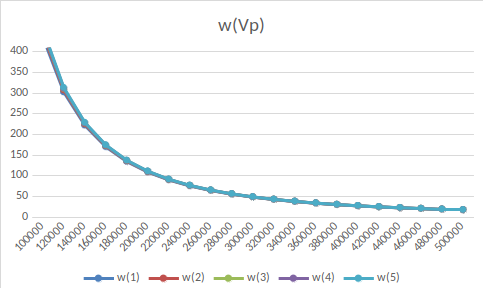
\includegraphics[scale=0.70]{img_1}}
	\caption{График зависимости $\omega(V_p)$ при $v_i = 0$}
	\label{img:1}
\end{figure}

\begin{figure}[H]
	\renewcommand{\figurename}{Рисунок}
	\centering{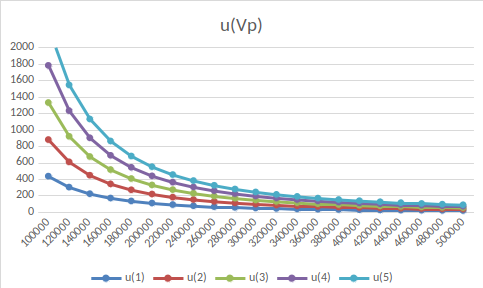
\includegraphics[scale=0.70]{img_2}}
	\caption{График зависимости $u(V_p)$ при $v_i = 0$}
	\label{img:2}
\end{figure}

\begin{figure}[H]
	\renewcommand{\figurename}{Рисунок}
	\centering{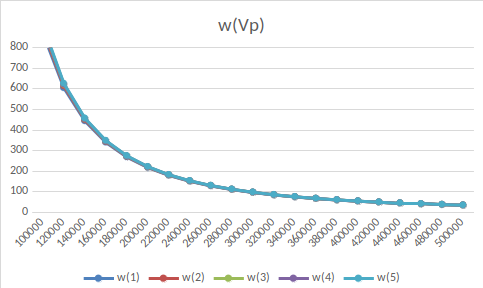
\includegraphics[scale=0.70]{img_3}}
	\caption{График зависимости $\omega(V_p)$ при $v_i = 1$}
	\label{img:3}
\end{figure}

\begin{figure}[H]
	\renewcommand{\figurename}{Рисунок}
	\centering{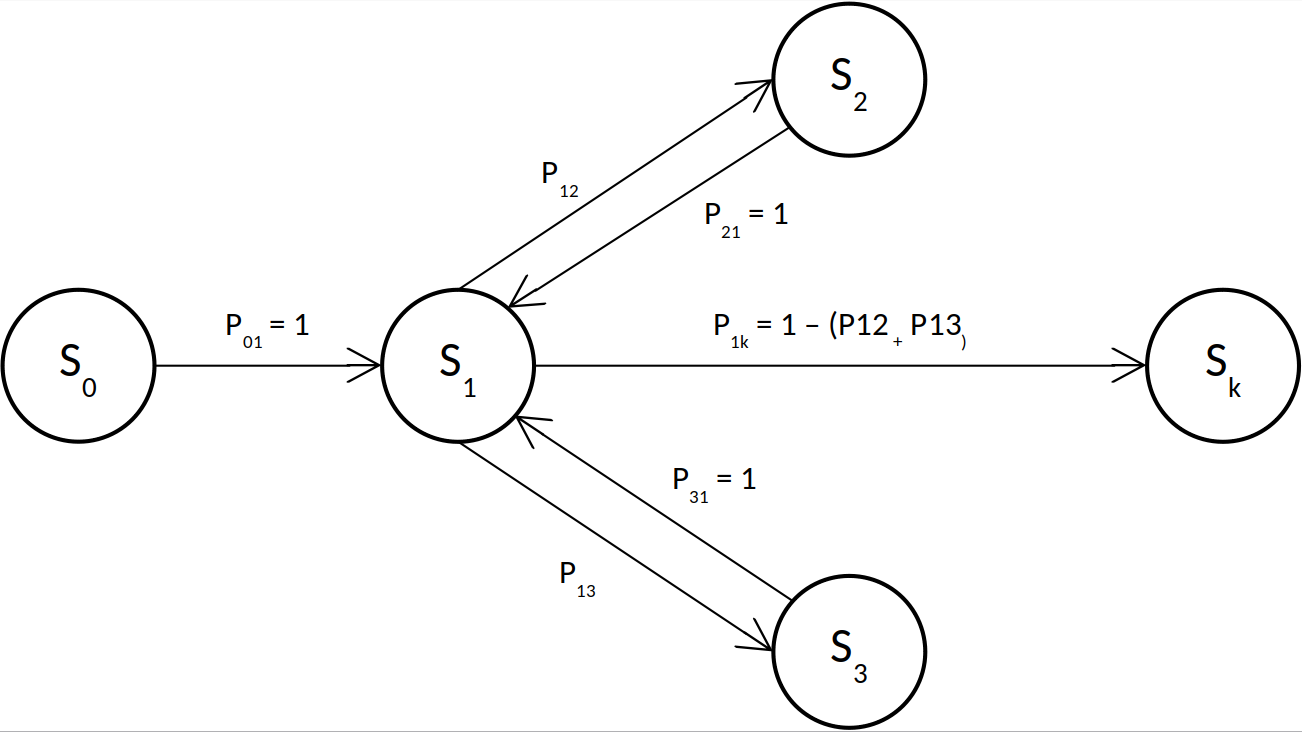
\includegraphics[scale=0.70]{img_4}}
	\caption{График зависимости $u(V_p)$ при $v_i = 1$}
	\label{img:4}
\end{figure}

\subsubsection*{Часть 2}

Длительность ожидания процесса обслуживания в системе при применении дисциплин обслуживания с абсолютными приоритетами рассчитывается по выражению:

\begin{align}
\omega_k = \frac{\vartheta_iR_{k-1}}{(1-R_k)} + \sum_{i=1}^{M}\frac{\rho_j\vartheta_j(1+v^2_i)}{2(1-R_k)(1-R_{k-1})}
\label{formul:5}
\end{align}

Время обслуживания потока в системе вычисляется по формуле:

\begin{align}
u_i = \sum_{j=1}^{k}\omega_j+\sum_{j=1}^{k}\vartheta_j
\label{formul:6}
\end{align}

\begin{align}
u_i = \sum_{i=1}^{M}u_j
\label{formul:7}
\end{align}

где
$M$ -- количество исполняемых в системе процессов, \\
$k$ -- количество ресурсов в системе, используемых при обслуживании процесса, \\
$\omega_j$ -- длительность ожидания $i$-го процесса обслуживания в $j$-ом ресурсе системы, \\
$\vartheta_j$ -- длительность обслуживания $i$-го процесса в $j$-ом ресурсе системы. \\

В таблицах \ref{table:7}-\ref{table:8} приведены результаты основных расчетов.

\begin{table}[H]
	\renewcommand{\tablename}{Таблица}
	\caption{Результаты вычислений при $v_i = 0$.}
	\begin{tabularx}{1\textwidth}{
			| >{\centering\arraybackslash}X
			| >{\centering\arraybackslash}X
			| >{\centering\arraybackslash}X
			| >{\centering\arraybackslash}X
			| >{\centering\arraybackslash}X
			| >{\centering\arraybackslash}X
			| >{\centering\arraybackslash}X
			| >{\centering\arraybackslash}X
			| >{\centering\arraybackslash}X
			| >{\centering\arraybackslash}X
			| >{\centering\arraybackslash}X |
		}
		\hline
		$V_p$ & $\omega(1)$ & $\omega(2)$ & $\omega(3)$ & $\omega(4)$ & $\omega(5)$ & $u(1)$ & $u(2)$ & $u(3)$ & $u(4)$ & $u(5)$ \\ \hline
		100000	&	435,148	&	639,238	&	1038,165	&	1089,638	&	1146,736	&	435,179	&	1074,448	&	2112,644	&	3202,313	&	4349,08	\\	\hline
		120000	&	301,872	&	442,198	&	717,505	&	752,84	&	791,396	&	301,898	&	744,122	&	1461,654	&	2214,519	&	3005,941	\\	\hline
		140000	&	221,619	&	323,985	&	525,354	&	551,101	&	578,862	&	221,641	&	545,648	&	1071,024	&	1622,147	&	2201,031	\\	\hline
		160000	&	169,583	&	247,539	&	401,2	&	420,791	&	441,724	&	169,602	&	417,16	&	818,379	&	1239,19	&	1680,934	\\	\hline
		180000	&	133,934	&	195,272	&	316,37	&	331,776	&	348,12	&	133,951	&	329,24	&	645,628	&	977,421	&	1325,559	\\	\hline
		200000	&	108,449	&	157,968	&	255,855	&	268,286	&	281,399	&	108,464	&	266,447	&	522,318	&	790,62	&	1072,034	\\	\hline
		220000	&	89,602	&	130,415	&	211,177	&	221,419	&	232,171	&	89,616	&	220,045	&	431,236	&	652,67	&	884,855	\\	\hline
		240000	&	75,273	&	109,489	&	177,257	&	185,84	&	194,816	&	75,285	&	184,788	&	362,057	&	547,911	&	742,74	\\	\hline
		260000	&	64,125	&	93,224	&	150,898	&	158,196	&	165,801	&	64,137	&	157,372	&	308,282	&	466,49	&	632,303	\\	\hline
		280000	&	55,282	&	80,331	&	130,01	&	136,29	&	142,817	&	55,293	&	135,635	&	265,656	&	401,957	&	544,785	\\	\hline
		300000	&	48,15	&	69,939	&	113,177	&	118,639	&	124,301	&	48,16	&	118,109	&	231,296	&	349,945	&	474,256	\\	\hline
		320000	&	42,313	&	61,44	&	99,413	&	104,207	&	109,165	&	42,323	&	103,773	&	203,196	&	307,412	&	416,586	\\	\hline
		340000	&	37,478	&	54,401	&	88,015	&	92,256	&	96,634	&	37,487	&	91,897	&	179,922	&	272,187	&	368,831	\\	\hline
		360000	&	33,426	&	48,506	&	78,471	&	82,25	&	86,144	&	33,434	&	81,949	&	160,429	&	242,688	&	328,84	\\	\hline
		380000	&	29,997	&	43,52	&	70,399	&	73,787	&	77,273	&	30,005	&	73,534	&	143,941	&	217,737	&	295,018	\\	\hline
		400000	&	27,07	&	39,265	&	63,512	&	66,567	&	69,705	&	27,078	&	66,351	&	129,87	&	196,445	&	266,158	\\	\hline
		420000	&	24,552	&	35,605	&	57,588	&	60,356	&	63,197	&	24,559	&	60,171	&	117,766	&	178,13	&	241,335	\\	\hline
		440000	&	22,369	&	32,434	&	52,455	&	54,976	&	57,56	&	22,376	&	54,817	&	107,279	&	162,262	&	219,829	\\	\hline
		460000	&	20,465	&	29,668	&	47,98	&	50,285	&	52,644	&	20,471	&	50,146	&	98,133	&	148,424	&	201,075	\\	\hline
		480000	&	18,794	&	27,241	&	44,054	&	46,169	&	48,333	&	18,8	&	46,048	&	90,108	&	136,283	&	184,623	\\	\hline
		500000	&	17,319	&	25,101	&	40,59	&	42,539	&	44,53	&	17,326	&	42,433	&	83,029	&	125,574	&	170,11	\\	\hline
	\end{tabularx}\label{table:7}
\end{table}

\begin{table}[H]
	\renewcommand{\tablename}{Таблица}
	\caption{Результаты вычислений при $v_i = 1$.}
	\begin{tabularx}{1\textwidth}{
			| >{\centering\arraybackslash}X
			| >{\centering\arraybackslash}X
			| >{\centering\arraybackslash}X
			| >{\centering\arraybackslash}X
			| >{\centering\arraybackslash}X
			| >{\centering\arraybackslash}X
			| >{\centering\arraybackslash}X
			| >{\centering\arraybackslash}X
			| >{\centering\arraybackslash}X
			| >{\centering\arraybackslash}X
			| >{\centering\arraybackslash}X |
		}
		\hline
		$V_p$ & $\omega(1)$ & $\omega(2)$ & $\omega(3)$ & $\omega(4)$ & $\omega(5)$ & $u(1)$ & $u(2)$ & $u(3)$ & $u(4)$ & $u(5)$ \\ \hline
		100000	&	870,296	&	1082,633	&	1487,873	&	1540,771	&	1601,466	&	870,327	&	1952,991	&	3440,894	&	4981,696	&	6583,193	\\	\hline
		120000	&	603,744	&	748,823	&	1027,756	&	1063,906	&	1104,519	&	603,77	&	1352,619	&	2380,401	&	3444,333	&	4548,878	\\	\hline
		140000	&	443,238	&	548,588	&	752,227	&	778,485	&	807,53	&	443,261	&	991,871	&	1744,12	&	2522,627	&	3330,18	\\	\hline
		160000	&	339,166	&	419,116	&	574,292	&	594,224	&	616,012	&	339,185	&	758,321	&	1332,632	&	1926,875	&	2542,907	\\	\hline
		180000	&	267,867	&	330,604	&	452,763	&	468,407	&	485,348	&	267,884	&	598,506	&	1051,286	&	1519,71	&	2005,076	\\	\hline
		200000	&	216,897	&	267,435	&	366,093	&	378,697	&	392,244	&	216,913	&	484,363	&	850,472	&	1229,184	&	1621,443	\\	\hline
		220000	&	179,203	&	220,781	&	302,121	&	312,492	&	323,57	&	179,217	&	400,012	&	702,148	&	1014,654	&	1338,238	\\	\hline
		240000	&	150,545	&	185,35	&	253,562	&	262,245	&	271,47	&	150,558	&	335,921	&	589,496	&	851,754	&	1123,237	\\	\hline
		260000	&	128,25	&	157,811	&	215,834	&	223,21	&	231,011	&	128,262	&	286,084	&	501,93	&	725,152	&	956,175	\\	\hline
		280000	&	110,564	&	135,982	&	185,941	&	192,283	&	198,967	&	110,575	&	246,568	&	432,52	&	624,814	&	823,792	\\	\hline
		300000	&	96,299	&	118,389	&	161,853	&	167,366	&	173,155	&	96,309	&	214,708	&	376,572	&	543,948	&	717,114	\\	\hline
		320000	&	84,627	&	104,001	&	142,16	&	146,996	&	152,059	&	84,637	&	188,647	&	330,817	&	477,823	&	629,891	\\	\hline
		340000	&	74,955	&	92,085	&	125,855	&	130,13	&	134,595	&	74,964	&	167,058	&	292,922	&	423,062	&	557,666	\\	\hline
		360000	&	66,851	&	82,106	&	112,201	&	116,009	&	119,977	&	66,86	&	148,974	&	261,184	&	377,202	&	497,187	\\	\hline
		380000	&	59,994	&	73,665	&	100,655	&	104,068	&	107,616	&	60,002	&	133,675	&	234,339	&	338,415	&	446,039	\\	\hline
		400000	&	54,14	&	66,462	&	90,804	&	93,88	&	97,072	&	54,148	&	120,617	&	211,429	&	305,316	&	402,396	\\	\hline
		420000	&	49,103	&	60,266	&	82,331	&	85,118	&	88,005	&	49,11	&	109,384	&	191,722	&	276,847	&	364,859	\\	\hline
		440000	&	44,738	&	54,897	&	74,991	&	77,527	&	80,151	&	44,745	&	99,649	&	174,647	&	252,181	&	332,34	\\	\hline
		460000	&	40,929	&	50,216	&	68,59	&	70,909	&	73,304	&	40,936	&	91,159	&	159,756	&	230,671	&	303,982	\\	\hline
		480000	&	37,588	&	46,108	&	62,975	&	65,103	&	67,298	&	37,594	&	83,709	&	146,691	&	211,8	&	279,105	\\	\hline
		500000	&	34,639	&	42,485	&	58,023	&	59,982	&	62,001	&	34,645	&	77,136	&	135,166	&	195,154	&	257,161	\\	\hline
	\end{tabularx}\label{table:8}
\end{table}


Графики зависимости при производительности процессора Vp, с относительными приоритетами представлены на рисунках \ref{img:5}-\ref{img:8}.

\begin{figure}[H]
	\renewcommand{\figurename}{Рисунок}
	\centering{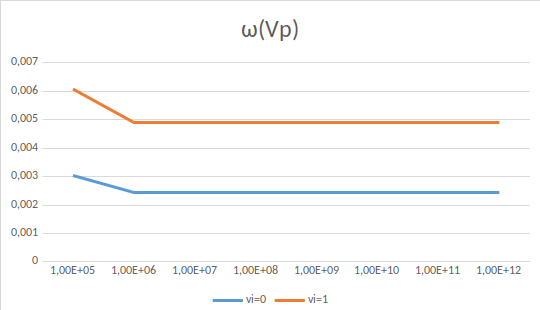
\includegraphics[scale=0.70]{img_5}}
	\caption{График зависимости $\omega(V_p)$ при $v_i = 0$}
	\label{img:5}
\end{figure}

\begin{figure}[H]
	\renewcommand{\figurename}{Рисунок}
	\centering{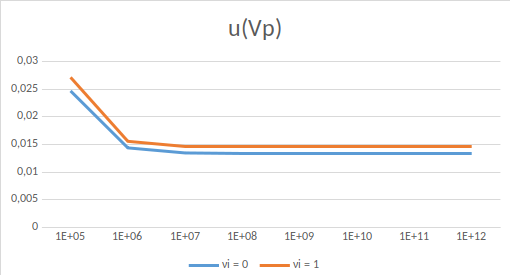
\includegraphics[scale=0.70]{img_6}}
	\caption{График зависимости $u(V_p)$ при $v_i = 0$}
	\label{img:6}
\end{figure}

\begin{figure}[H]
	\renewcommand{\figurename}{Рисунок}
	\centering{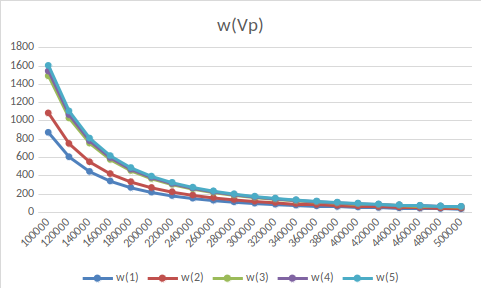
\includegraphics[scale=0.70]{img_7}}
	\caption{График зависимости $\omega(V_p)$ при $v_i = 1$}
	\label{img:7}
\end{figure}

\begin{figure}[H]
	\renewcommand{\figurename}{Рисунок}
	\centering{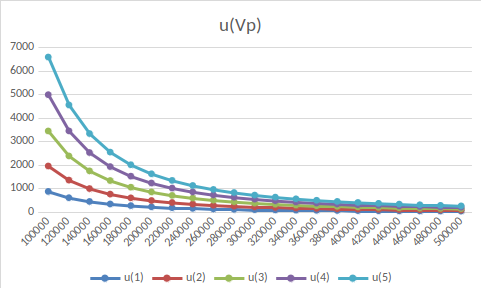
\includegraphics[scale=0.70]{img_8}}
	\caption{График зависимости $u(V_p)$ при $v_i = 1$}
	\label{img:8}
\end{figure}

\newpage



